\documentclass[11pt,a4paper]{article}
\usepackage[margin=2.4cm]{geometry}
\usepackage{amsmath,amssymb,amsthm,mathtools}
\usepackage[protrusion=true,expansion=false]{microtype}
\usepackage{booktabs,enumitem}
\usepackage{placeins}
\usepackage{tikz}
\usetikzlibrary{arrows.meta,positioning,calc,fit,backgrounds}
\definecolor{tierspend}{RGB}{200,60,60}
\definecolor{tierfull}{RGB}{210,140,40}
\definecolor{tierin}{RGB}{60,130,180}
\definecolor{tierrecv}{RGB}{70,150,90}
\usepackage[colorlinks=true,linkcolor=blue!50!black,citecolor=blue!50!black,urlcolor=blue!50!black]{hyperref}

\emergencystretch=3em
\hbadness=10000
\hfuzz=2pt

\newtheorem{theorem}{Theorem}[section]
\newtheorem{lemma}[theorem]{Lemma}
\newtheorem{proposition}[theorem]{Proposition}
\newtheorem{corollary}[theorem]{Corollary}
\theoremstyle{definition}
\newtheorem{definition}[theorem]{Definition}
\newtheorem{construction}[theorem]{Construction}
\newtheorem{assumption}[theorem]{Assumption}
\newtheorem{remark}[theorem]{Remark}
\newtheorem{example}[theorem]{Example}

\newcommand{\F}{\mathbb{F}}
\newcommand{\Z}{\mathbb{Z}}
\newcommand{\N}{\mathbb{N}}
\newcommand{\G}{\mathbb{G}}
\newcommand{\E}{\mathbb{E}}
\newcommand{\PP}{\mathbb{P}}
\renewcommand{\Pr}{\mathrm{Pr}}
\newcommand{\Fp}{\F_p}
\newcommand{\Fq}{\F_q}
\newcommand{\ip}[2]{\langle #1,\, #2 \rangle}
\newcommand{\Comm}{\mathsf{Commit}}
\newcommand{\Open}{\mathsf{Open}}
\newcommand{\Setup}{\mathsf{Setup}}
\newcommand{\Verify}{\mathsf{Verify}}
\newcommand{\negl}{\mathsf{negl}}
\newcommand{\poly}{\mathsf{poly}}
\newcommand{\PPT}{\mathsf{PPT}}
\newcommand{\Adv}{\mathcal{A}}
\newcommand{\Prov}{\mathcal{P}}
\newcommand{\Ver}{\mathcal{V}}
\newcommand{\Sim}{\mathcal{S}}
\newcommand{\Ext}{\mathcal{E}}
\newcommand{\Rel}{\mathcal{R}}
\newcommand{\Lang}{\mathcal{L}}
\newcommand{\nfsym}{\mathsf{nf}}
\newcommand{\cmsym}{\mathsf{cm}}
\newcommand{\cmx}{\mathsf{cmx}}
\newcommand{\cvsym}{\mathsf{cv}}
\newcommand{\rk}{\mathsf{rk}}
\newcommand{\Pallas}{\ensuremath{\mathsf{Pallas}}}
\newcommand{\Vesta}{\ensuremath{\mathsf{Vesta}}}
\newcommand{\Ep}{\ensuremath{\mathcal{E}}}
\newcommand{\NoteCommit}{\ensuremath{\mathsf{NoteCommit}}}
\newcommand{\Sinsemilla}{\ensuremath{\mathsf{Sinsemilla}}}
\newcommand{\ShortCommit}{\ensuremath{\mathsf{ShortCommit}}}
\newcommand{\CommitIvk}{\ensuremath{\mathsf{Commit}^{\mathsf{ivk}}}}
\newcommand{\Extract}{\ensuremath{\mathsf{Extract}}}
\newcommand{\Acc}{\ensuremath{\mathsf{Acc}}}
\newcommand{\GroupHash}{\ensuremath{\mathsf{GroupHash}}}
\newcommand{\ask}{\ensuremath{\mathsf{ask}}}
\newcommand{\aksym}{\ensuremath{\mathsf{ak}}}
\newcommand{\nksym}{\ensuremath{\mathsf{nk}}}
\newcommand{\ivk}{\ensuremath{\mathsf{ivk}}}
\newcommand{\fvk}{\ensuremath{\mathsf{fvk}}}
\newcommand{\ovk}{\ensuremath{\mathsf{ovk}}}
\newcommand{\dk}{\ensuremath{\mathsf{dk}}}
\newcommand{\pkd}{\ensuremath{\mathsf{pk_d}}}
\newcommand{\gd}{\ensuremath{\mathsf{g_d}}}
\newcommand{\rcv}{\ensuremath{\mathsf{rcv}}}
\newcommand{\rcm}{\ensuremath{\mathsf{rcm}}}
\newcommand{\rivk}{\ensuremath{\mathsf{r_{ivk}}}}
\newcommand{\rsk}{\ensuremath{\mathsf{rsk}}}

\renewenvironment{abstract}{%
  \small\begin{center}{\bfseries\abstractname}\end{center}\medskip\noindent\ignorespaces
}{\par\medskip}

\title{\textbf{\Huge PQ Guide}\\[6pt]\large Post-quantum Zcash: the cross-layer assumption inventory, the reversibility divide, and the migration surface}
\author{m@rek.onl}
\date{}
\begin{document}
\maketitle
\thispagestyle{empty}
\begin{abstract}
This volume of \emph{The Zcash Arboretum} assembles the post-quantum
picture that no single layer can see. It inventories
every deployed cryptographic surface --- the shielded core, the
transparent layer, the Sprout and Sapling remnants, proof of work, and
the frontier protocols --- against the two quantum algorithms that
matter, and sorts every exposure along one axis: \emph{retroactive}
(damage accruing now, in recorded data) against \emph{prospective}
(exploitable only once a quantum adversary exists, and mitigable by
switching off in time). It quantifies quantum mining through the
\emph{Consensus Guide}'s own tables, situates ZIP-2005's
recoverability-not-resistance strategy and its stated gaps, computes the
migration arithmetic against the published NIST standards, and registers
the distance between public statements and the repositories --- which
contain, at the pinned commits, no deployed post-quantum cryptography at
all. The Orchard-core analysis is the \emph{Ironwood Guide}'s; this
volume cites it and extends the frame to everything else.
\end{abstract}
\clearpage
\tableofcontents
\clearpage

\section{Scope, method, and the two clocks}\label{sec:pq-scope}

Every volume below this one proves what an assumption buys while it
holds. This volume asks the cross-layer question: what happens to each
purchase when the assumption falls to a quantum adversary --- and, since
the falls are not simultaneous in their \emph{effects}, in what order
the damage arrives. The treatment is an inventory and a synthesis, not a
re-derivation: the deep analysis of the Orchard core is the
\emph{Ironwood Guide}'s (\S``Post-quantum security of the Orchard
protocol''), the cryptographic definitions are the \emph{Crypto
Guide}'s, and this volume constructs only what no lower volume owns ---
the cross-layer inventory, the quantum-mining analysis, and the
migration arithmetic.

Two quantum algorithms carry the whole subject. Shor's algorithm solves
the discrete-logarithm problem in polynomial time in \emph{any} group,
elliptic curves included, taking DLP, CDH, and DDH with it (\emph{Crypto
Guide}, \S``The quantum caveat: Shor's algorithm''); every
discrete-log-based object in Zcash --- which is nearly every
asymmetric object --- fails completely against it. Grover's algorithm
gives a quadratic speedup on unstructured search and nothing more:
symmetric primitives and hashes retain half their security exponent, a
margin the deployed 256-bit parameters absorb. The standing premise,
inherited from the same section, is that no cryptographically relevant
quantum computer (CRQC) exists today; nothing in this volume predicts
when one will, and every claim is conditioned explicitly on that event.

\subsection{The reversibility axis}\label{sec:pq-axis}

One distinction organises everything, and the series already owns its
two halves. The \emph{Crypto Guide}'s remark ``Two regimes, two failure
modes'' (\S``Incompatibility of perfect hiding and perfect binding'')
observes the asymmetry: a computationally \emph{binding} commitment
leaves a future solver able to change a committed value, while a
computationally \emph{hiding} one loses everlasting secrecy the day the
assumption falls, for everything ever recorded. Which direction each
failure \emph{points in time} is the \emph{Ironwood Guide}'s
operational recasting, and it turns the asymmetry into a test: a break
is \emph{prospective} when its
exploitation requires a validator to \emph{accept} a forged object,
because acceptance happens at the current chain height --- disabling
the protocol first removes every future acceptance event, so forking in
time is a complete mitigation; a break is \emph{retroactive} when
recorded data itself becomes exploitable, and no consensus change can
help, because the adversary's copy of the chain is beyond the
protocol's reach.

Along that axis, the deployed protocol has exactly one retroactive
break --- harvest-now-decrypt-later against note encryption --- and a
stack of prospective ones; Section~\ref{sec:pq-inventory} walks the full
inventory. Figure~\ref{fig:pq-axis} draws the divide.

\begin{figure}[ht]
\centering
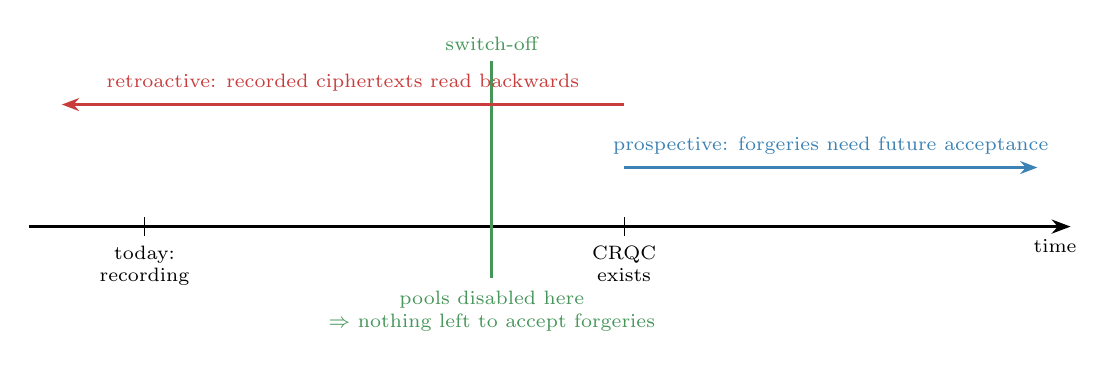
\begin{tikzpicture}[
  x=1.05cm, y=1cm,
  evt/.style={font=\scriptsize, align=center},
  lbl/.style={font=\scriptsize},
]
% time axis
\draw[-{Stealth[length=2.4mm]}, thick] (0,0) -- (12.6,0)
  node[below right=1pt and -6mm, font=\scriptsize] {time};
\foreach \x/\t in {1.4/{today:\\recording}, 7.2/{CRQC\\exists}}
  \draw (\x,0.12) -- (\x,-0.12) node[below, evt] {\t};
% switch-off wall
\draw[very thick, tierrecv] (5.6,-0.65) -- (5.6,2.1)
  node[above, evt, text=tierrecv] {switch-off};
% retroactive channel: arrow from CRQC pointing BACK over recorded data
\draw[{Stealth[length=2.2mm]}-, thick, tierspend]
  (0.4,1.55) -- (7.2,1.55);
\node[lbl, text=tierspend, anchor=south] at (3.8,1.6)
  {retroactive: recorded ciphertexts read backwards};
% prospective channel: forward from CRQC, blocked by wall if wall < CRQC
\draw[-{Stealth[length=2.2mm]}, thick, tierin]
  (7.2,0.75) -- (12.2,0.75);
\node[lbl, text=tierin, anchor=south] at (9.7,0.8)
  {prospective: forgeries need future acceptance};
\node[lbl, text=tierrecv, anchor=north, align=center] at (5.6,-0.7)
  {pools disabled here\\$\Rightarrow$ nothing left to accept forgeries};
\end{tikzpicture}
\caption{The reversibility divide. A prospective break (blue) needs a
validator to accept a forged object after a CRQC exists; switching the
vulnerable protocols off first (green) leaves it nothing to act on. The
retroactive channel (red) runs the other way: ciphertexts recorded today
are read by tomorrow's adversary, and no protocol change reaches the
adversary's copy of the chain.}
\label{fig:pq-axis}
\end{figure}

\subsection{Sources and their standing}\label{sec:pq-sources}

Table~\ref{tab:pq-sources} lists the sources. Normative weight is
ZIP-2005's (Proposed) and the cited Final ZIPs'; the NIST standards are
normative for their own schemes and serve here only as the published
size and security baselines; everything else is analysis or code.
Worked numbers are computed by script
(\texttt{.wip/pq-drafts/compute.py}, whose output is the source of
every numeric claim here); deployed-behaviour claims cite crate, file,
and line at the pinned commits.

\begin{table}[ht]
\centering
\small
\begin{tabular}{@{}lll@{}}
\toprule
Source & Role & Pin \\
\midrule
ZIP-2005 (Ironwood Quantum Recoverability) & Proposed & \texttt{zips} \texttt{69610984} \\
ZIPs 213, 229, 258, 326; ZIP-209 & normative/draft & same pin \\
FIPS 203/204/205 (ML-KEM, ML-DSA, SLH-DSA) & published 2024-08-13 & retrieved 2026-08-19 \\
Ben-Sasson et al., ePrint 2018/046; ethSTARK 2021/582 & analysis & retrieved 2026-08-19 \\
Aggarwal et al., arXiv:1710.10377 & analysis (2017) & retrieved 2026-08-19 \\
\textsf{zebra} & deployed validator & \texttt{8e9ff3b2c} \\
\textsf{reddsa} 0.5.1 / \textsf{halo2\_proofs} 0.3.2 / \textsf{orchard} 0.15.3 & deployed crates & Cargo.lock \\
\textsf{zebra-crosslink} & prototype & \texttt{6d02a1b8} \\
\bottomrule
\end{tabular}
\caption{Sources. The quantum-relevant repository state was swept at
these pins: the zips repository and the protocol specification contain
zero occurrences of ML-KEM, Kyber, ML-DSA, Dilithium, SPHINCS, Falcon,
or ``lattice''; the sole post-quantum bytes in any ecosystem checkout
are an inert, feature-gated transitive dependency
(Section~\ref{sec:pq-register}).}
\label{tab:pq-sources}
\end{table}

\FloatBarrier

\section{The inventory: every deployed surface, sorted}\label{sec:pq-inventory}

Table~\ref{tab:pq-inventory} is the volume's spine: every cryptographic
surface a mainnet validator enforces today (with the one frontier
prototype, Crosslink, marked as such), its assumption, what a CRQC
does to it, and on which side of the divide the damage falls. The
Orchard-core rows compress the \emph{Ironwood Guide}'s five-subsection
analysis and the committed inventory it rests on; the remaining rows are
this volume's. The subsections walk the table by failure mode.

\begin{table}[ht]
\centering
\footnotesize
\setlength{\tabcolsep}{4pt}
\begin{tabular}{@{}p{3.4cm}p{3.2cm}p{5.6cm}l@{}}
\toprule
Surface & Assumption & Consequence of a CRQC & Side \\
\midrule
Note encryption (all shielded pools) & DH on the pool's curve &
decrypt every recorded ciphertext to a \emph{known address}: amounts,
memos, full receiving history & \textbf{retro} \\
\addlinespace[2pt]
Sinsemilla commitments (\NoteCommit, \CommitIvk, MerkleCRH) & Pallas
DLP (binding) & equivocate openings: forge notes, fake Merkle paths,
Spendability attacks & prosp. \\
Value commitments + binding signature & Pallas DLP & reopen
$\cvsym$ to any value; forge balance --- silent inflation, bounded only
by the ZIP-209 turnstiles & prosp. \\
RedPallas spend authorisation & Pallas DLP (ROM) & forge spend-auth
from public $\rk$; with forged proofs, theft & prosp. \\
Halo 2 IPA proof soundness & Vesta DLP (ROM) & prove arbitrary false
Action statements --- the most concentrated point & prosp. \\
Sapling stack (Groth16, RedJubjub, Jubjub DH) & BLS12-381 / Jubjub
DLP & one logarithm forges the whole pool's integrity & prosp. \\
Sprout stack (Groth16, Ed25519 \texttt{JoinSplitSig}) & BLS12-381 /
Curve25519 DLP & JoinSplit statements and signatures forgeable & prosp. \\
Transparent scripts (ECDSA, secp256k1) & secp256k1 DLP & spend any
output whose public key is exposed & prosp. \\
Crosslink finalizer votes (prototype; ed25519) & Curve25519 DLP &
forge roster signatures --- the finality premise itself
(\S\ref{sec:pq-frontier}) & prosp. \\
\addlinespace[2pt]
Proof of work (Equihash + SHA-256d filter) & generic search & Grover:
quadratic speedup, heavily damped (\S\ref{sec:pq-mining}) & neither \\
BLAKE2b backbone, ZIP-32 tree, Poseidon-as-PRF & symmetric / hash &
security exponent halves; parameters absorb it & survives \\
\bottomrule
\end{tabular}
\caption{The deployed surfaces under a CRQC. ``retro'' = retroactive
(recorded data becomes exploitable; no protocol change helps);
``prosp.'' = prospective (requires future validator acceptance;
switch-off before a CRQC is a complete mitigation, with the residues of
Section~\ref{sec:pq-2005}). Orchard-core rows: \emph{Ironwood Guide},
\S``Post-quantum security of the Orchard protocol''.}
\label{tab:pq-inventory}
\end{table}

\subsection{The retroactive wound}\label{sec:pq-retro}

One row of Table~\ref{tab:pq-inventory} is red, and it is the one
accruing damage today. Every shielded output ever recorded carries an
ephemeral key and a ciphertext; for the Orchard pools, one Shor
logarithm per \emph{address} yields the incoming viewing key
($\ivk = \log_{\gd} \pkd$), after which the adversary runs the
recipient's own trial-decryption loop over the whole recorded chain ---
amounts, memos, and the complete receiving history of that address,
forever. The full anatomy, and the two structural limits --- the
attack is keyed by the address, and it confers viewing rather than
spending --- are the \emph{Ironwood Guide}'s (\S``The retroactive
break: harvest now, decrypt later against note encryption''). Three
extensions belong to the cross-layer frame:

\begin{itemize}[leftmargin=*]
\item \emph{Every pool, not one.} Sapling and Sprout note encryption
are equally DH-keyed and their ciphertexts equally recorded; ZIP-2005
itself states that note encryption for the ``Ironwood, Orchard,
Sapling, and Sprout pools'' is subject to harvest-now-decrypt-later
given ciphertext and receiver address. The corpus is the union of every
shielded output since 2016, growing with each block --- including
Ironwood's, whose recoverability machinery deliberately excludes
privacy (Section~\ref{sec:pq-2005}).
\item \emph{Where the address is already public, so is the history.}
Shielded coinbase outputs must decrypt under the all-zero outgoing
viewing key (\emph{Ironwood Guide}, \S``How value enters the pool''),
so their contents were never confidential; and ZIP-213 itself advises
miners who rely on the ``post-quantum privacy'' of an address to use a
coinbase-specific one --- the ZIP's only pre-2005 use of the phrase.
\item \emph{What stays dark even then.} Without the address, the
recorded chain leaks nothing to an unbounded adversary: value
commitments are perfectly hiding, the spend-auth randomiser masks
$\ask$ information-theoretically, and proof transcripts are
statistically simulatable (\emph{Ironwood Guide},
\S``Prospective breaks: the discrete-logarithm integrity stack'',
closing paragraph; the underlying theorems are the \emph{Crypto
Guide}'s and \emph{Halo 2 Guide}'s). The retroactive channel is
address-shaped, exactly.
\end{itemize}

\subsection{The prospective integrity stack}\label{sec:pq-prosp}

Every other broken row fails forward, and for the Orchard core the
\emph{Ironwood Guide} already orders the dominoes --- Sinsemilla
binding, value commitments, RedPallas, and the IPA's knowledge
soundness, the last ``the single most concentrated failure point''
because every other item's exploitation route runs through it. The
cross-layer frame adds four members the core analysis does not cover.

\paragraph{The transparent layer.} Script signatures are ECDSA over
secp256k1 (specification \S`Signature'), verified in deployment by the
retired \textsf{zcashd}'s own C++ interpreter bundled as a crate
(\textsf{libzcash\_script}, \texttt{depend/zcash/src/pubkey.cpp:23--42},
driven from \texttt{zebra-script/src/lib.rs:62--76}). Exposure is
per-output and public-key-shaped: an address spent from before has its
key on chain --- forgeable the day a CRQC exists, no acceptance of any
new object required beyond an ordinary transaction; an unspent P2PKH or
P2SH output exposes only a hash until its first spend, leaving a
between-broadcast-and-confirmation window thereafter (ZIP-2005's own
analysis, which also notes P2PK and bare multisig were never produced
by Zcash wallets). Two special cases sharpen the picture. The deferred
lockbox is secured by consensus accounting alone --- the pool has no
output, no address, and no key, so a CRQC finds nothing to steal there;
only a consensus change moves it. The 78{,}750~ZEC already disbursed
under ZIP-271, by contrast, sit in a 2-of-3 P2SH multisig whose
extended public keys are published in the ZIP itself, so hash-hiding
provides those particular funds no pre-spend quantum cover.

\paragraph{The Sprout remnant.} Version-4 transactions remain
consensus-valid --- ZIP-2003 (disallowing them) is Draft and absent
from the NU6.3 upgrade list --- so \textsf{zebra} still runs Groth16
JoinSplit verification and Ed25519 \texttt{JoinSplitSig} checks
(\texttt{zebra-consensus/src/transaction.rs:1230, 1265--1268};
\textsf{ed25519-zebra}). ZIP-2005 states the consequence plainly: the
broken proof system suffices to forge JoinSplit statements, and both
Sprout signature layers are forgeable. One logarithm on BLS12-381
undoes Sprout and Sapling integrity alike; one on Pallas/Vesta undoes
Orchard and Ironwood.

\paragraph{The Sapling pool.} Groth16 over BLS12-381 with RedJubjub
authorisation and Jubjub key agreement --- the same stack shape as
Orchard with every assumption transplanted, and deliberately
\emph{excluded} from ZIP-2005's recoverability (its stated
analysis-economy decision). Sapling funds therefore face the harder
edge of the strategy: prospective integrity failure like Orchard's,
but no recovery door --- migration before switch-off is the only
remedy the design offers.

\paragraph{The finality prototype.} Crosslink's roster votes are plain
ed25519 signatures under long-lived finalizer keys
(Section~\ref{sec:pq-frontier}); a CRQC forges the very signatures
whose aggregation is supposed to make history \emph{assuredly} final.

\subsection{The surviving backbone}\label{sec:pq-backbone}

What remains standing is exactly what ZIP-2005 builds on. The BLAKE2b
expansion registry, the hardened-only ZIP-32 key tree (whose
$\geq$256-bit seed requirement the ZIP text motivates by quantum
analysis), Poseidon in its PRF role, and the consensus hashes ---
SHA-256d in the difficulty filter, BLAKE2b in the ZIP-221 history tree
--- face only generic speedups: Grover halves the security exponent,
$2^{256} \to 2^{128}$, a margin the parameters absorb, and the sharper
quantum collision algorithms remain memory-bound curiosities (the
\emph{Ironwood Guide}'s \S``Primitives facing only generic speedups''
carries the careful statement, including its best-known-not-provably-best
flag). The load-bearing consequence, stated there and relied on
everywhere in Section~\ref{sec:pq-2005}: because key derivation is
purely symmetric, \emph{ownership remains provable after the assumption
that made it enforceable has fallen} --- the seed still derives the
keys; what is lost is only the DL-based machinery for exercising them.

\section{Quantum mining}\label{sec:pq-mining}

The one broken row that is neither retroactive nor prospective is proof
of work, because Grover attacks it and Grover only halves an exponent.
No volume of the series analyses this; the \emph{Consensus Guide} builds
the double-spend model on a fixed hashrate share $q$ but never asks what
a quantum miner does to $q$. This section closes that gap, reusing that
volume's machinery.

The gated quantity is a hash lottery: a block is valid when the
SHA-256d of its header falls below the target (\emph{Consensus Guide},
\S``Equihash and the memoryless model''; the difficulty filter is
deployed at \texttt{zebra-consensus/src/block/\allowbreak
check.rs:112--139} over the SHA-256d header hash). That filter is
unstructured search, exactly Grover's domain --- with three deflations
that the honest statement must carry, and a fourth specific to Zcash:
the candidates a classical Equihash miner feeds the filter come from
Wagner-structured solver runs, not brute force, so a quantum miner
would have to embed that structured search in its Grover oracle to gain
on the whole pipeline rather than on the filter alone.

\begin{remark}[The three deflations]\label{rem:pq-grover-caveats}
Aggarwal, Brennen, Lee, Santha, and Tomamichel (arXiv:1710.10377, 2017)
state them (published in \emph{Ledger}, 2018). \emph{Quadratic, not
exponential}: Grover ``can perform the hashcash [proof of work] by
performing quadratically fewer hashes'', so $N$ classical trials become
$\sqrt{N}$ --- a square root, not a collapse. \emph{Gate speed}: at 2017
difficulty ``the extreme speed of
current specialized ASIC hardware $\ldots$ coupled with much slower
projected gate speeds for current quantum architectures, essentially
negates this quadratic speedup $\ldots$ giving quantum computers no
advantage''; only a hypothesised 100~GHz gate speed would let a quantum
miner ``solve the [proof of work] about 100 times faster''.
\emph{Parallelisation}: Grover parallelises badly --- across $d$
processors the search \emph{time} falls only as $\sqrt{d}$, against the
linear scaling a classical pool enjoys, so a quantum miner cannot buy
back the speed by fanning out. The date matters: these are 2017
projections, cited as the structural shape of the advantage, not a
forecast.
\end{remark}

The model needs no rebuilding, only a reading. A quantum miner is one
whose search is faster per unit hardware; fold the advantage into an
effective speed multiplier $g$ on the attacker's raw hashing, and the
\emph{Consensus Guide}'s hashrate share becomes
\[
  q_{\mathrm{eff}}(f, g) \;=\; \frac{g f}{g f + (1 - f)}
  \qquad \text{for a raw share } f \text{ of the total hashing rate}
\]
(the honest remainder being $1 - f$; at $g = 1$, $q_{\mathrm{eff}} = f$,
the plain hashrate share of that volume),
after which every result of that volume applies to $q_{\mathrm{eff}}$
unchanged --- its double-spend probability $r(q, n)$, its confirmation
tables, its majority threshold at $q = \tfrac12$. Table~\ref{tab:pq-qeff}
computes the effect (by script, from that volume's $r(q, n)$).

\begin{table}[ht]
\centering
\small
\begin{tabular}{@{}r r r r r@{}}
\toprule
raw $f$ & speedup $g$ & $q_{\mathrm{eff}}$ & $r(q_{\mathrm{eff}},6)$ &
$r(q_{\mathrm{eff}},10)$ \\
\midrule
$1\%$  & $1$   & $0.010$ & ${<}10^{-6}$ & ${<}10^{-6}$ \\
$1\%$  & $10$  & $0.092$ & $0.037\%$    & $0.0004\%$ \\
$1\%$  & $100$ & $0.503$ & $100\%$      & $100\%$ \\
$5\%$  & $10$  & $0.345$ & $28.0\%$     & $16.0\%$ \\
$10\%$ & $2$   & $0.182$ & $1.44\%$     & $0.15\%$ \\
$10\%$ & $10$  & $0.526$ & $100\%$      & $100\%$ \\
$25\%$ & $2$   & $0.400$ & $49.3\%$     & $37.2\%$ \\
\bottomrule
\end{tabular}
\caption{A per-unit mining speedup $g$ applied to an attacker's raw
share $f$ of total hashing, and the resulting double-spend success
against $6$ and $10$ confirmations, computed by script from the
\emph{Consensus Guide}'s $r(q, n)$. The threshold that matters is the
majority line: $q_{\mathrm{eff}} > \tfrac12$ iff $g > (1 - f)/f$, i.e.\
a $10\%$ miner needs $g > 9$, a $5\%$ miner $g > 19$, a $1\%$ miner
$g > 99$.}
\label{tab:pq-qeff}
\end{table}

The reading is reassuring and precise. Grover halves the search
\emph{exponent} --- a quadratic search over an $H$-bit target is
$2^{H/2}$ rather than $2^H$ trials --- so the ideal \emph{rate}
multiplier grows as the square root of the expected trial count, not to
some fixed bound; what keeps the realised $g$ small is not the algorithm
but the gate-speed deflation of Remark~\ref{rem:pq-grover-caveats} (no
advantage at 2017 parameters, about $100$ under its hypothesised
$100$~GHz gates). The table spans that uncertainty deliberately. Read
at a modest near-term operating point of $g = 2$, even a $25\%$ raw
share reaches only $q_{\mathrm{eff}} = 0.40$, short of majority, and a
$10\%$ share sits at $r = 1.44\%$ over six confirmations; read at the
$100$~GHz hypothesis, a $g = 100$ miner is over the majority line from a
$1\%$ raw share. Either way a quantum miner rewrites the double-spend
arithmetic the way any faster miner does --- by raising $q$ --- and
proof of work degrades gracefully where the signature layers shatter.
This asymmetry is the same one Aggarwal et
al.\ draw for Bitcoin: the proof of work is ``relatively resistant'',
the signatures ``much more at risk''.

\begin{remark}[Lumpy progress, quantum edition]\label{rem:pq-lumpy}
The \emph{Consensus Guide}'s difficulty remark (\S``Difficulty in
motion'') shows that the overtake probability of a work-scored race
depends on the \emph{granularity} of progress, but its mechanism is
work \emph{per block} under difficulty manipulation --- which quantum
mining leaves unchanged, since a quantum miner's blocks carry the same
work as anyone else's at the network difficulty. A distinct channel
does remain: the \emph{inter-arrival} dispersion of a quantum miner's
block discoveries need not match the memoryless stream the model
assumes, and its direction (Grover completions may be more regular, not
less) is unanalysed here. It is flagged as the one place the reduction
to $q_{\mathrm{eff}}$ is not exact; the effect is second-order against
the deflations above.
\end{remark}

\section{The frontier surfaces}\label{sec:pq-frontier}

Two designs beyond the deployed core carry quantum-relevant structure
their own volumes state but do not analyse; the closing volume must.

\paragraph{Crosslink finality.} The trailing-finality prototype
(\emph{Crosslink Guide}, \S``Finalizer keys'') gives each finalizer a
single ed25519 key and makes a roster vote a plain ed25519 signature
over a $76$-byte payload (\texttt{zebra-crosslink/src/lib.rs:2011}
onward, at the prototype pin). The construction's whole point is to
convert proof-of-work's \emph{probabilistic} finality --- the $r(q, n)$
of Section~\ref{sec:pq-mining} --- into \emph{assured} finality by BFT
signatures. Under a CRQC that inverts: the finalizer keys are long-lived
roster identities that must stay secret indefinitely, and Shor forges
their signatures, so an adversary manufactures the two-thirds agreement
the BFT layer contributes. The prototype sources no threshold or
post-quantum design for these keys anywhere; the \emph{FROST Guide}'s
own inference (\S``Crosslink finalizer keys'') is that the natural
fit would be \textsf{FROST}(Ed25519, SHA-512) --- itself classical.
Crosslink's safety is a disjunction --- assured finality from the
proof-of-work prefix \emph{or} the BFT agreement (\emph{Crosslink
Guide}, \S``The safety theorems and their assumptions'') --- so a CRQC
does not erase finality outright; it deletes the BFT half of that
disjunction, collapsing the guarantee back onto the probabilistic
proof-of-work floor of Section~\ref{sec:pq-mining}. The upgrade the BFT
layer was meant to buy is exactly what a quantum adversary forges.

\paragraph{FROST threshold spending.} FROST rerandomised RedPallas is
the deployed threshold path, and it is DL-based like everything it
signs for (\textsf{reddsa}, \texttt{src/frost/redpallas.rs}: group
Pallas, an aggregated signature verifying as an ordinary RedPallas
spend-auth). ZIP-2005 extends its quantum-recovery mechanism to FROST
through a shared quantum spending key $\mathsf{qsk}$ that every
participant holds (\emph{FROST Guide}, \S``Custody of the ZIP-2005
quantum spending key'') --- which defeats the $t$-of-$n$ threshold
against a quantum adversary, since one compromised participant's
$\mathsf{qsk}$ suffices. The ZIP accordingly recommends migrating
FROST-held funds to a genuinely post-quantum threshold protocol ``as
soon as'' one exists; none does, and the derivation-agreement gap
(participants must privately agree a seed $\mathsf{sk}$, with no
protocol for it) remains open. The frontier inherits the core's
strategy and its unfinished edges both.

\section{ZIP-2005 in the cross-layer frame}\label{sec:pq-2005}

The deployed answer to all of this is one Proposed ZIP, and the
\emph{Ironwood Guide} anatomises its mechanism (\S``ZIP-2005: quantum
recoverability of Ironwood notes'') --- the $\mathtt{0x0B}$-tagged
hashed derivation that makes each Ironwood note's commitment
\emph{conditionally} post-quantum-binding, the $\mathsf{qsk}$ path for
non-seed keys, the non-normative Recovery Statement, and the QROM
security bounds. This volume adds only the cross-layer placement.

\emph{What it is.} A recoverability mechanism, not a resistance one:
ZIP-2005 states in terms that it ``does not by itself make the protocol
secure against quantum adversaries'', and arranges instead that
Ironwood-pool funds survive the eventual, necessary switch-off of the
DL-based pools. Its lever is the surviving backbone of
Section~\ref{sec:pq-backbone}: because the seed still derives every key
symmetrically \emph{and} the $\mathtt{0x0B}$-tagged hashed derivation
makes each Ironwood note commitment conditionally post-quantum-binding,
a future Recovery Protocol can let a holder prove ownership and re-mint
under post-quantum assumptions --- ownership outliving enforceability.

\emph{What it is not}, mapped onto the inventory
(Table~\ref{tab:pq-inventory}):

\begin{itemize}[leftmargin=*]
\item \emph{The retroactive wound is untouched.} Privacy is an explicit
non-requirement; harvest-now-decrypt-later persists for every pool
including Ironwood, with mitigations only ``under consideration''. The
one break that is bleeding today gets nothing.
\item \emph{Several surfaces are out of scope entirely.} Transparent
ECDSA is deferred to a Reserved ZIP-2007 stub; and the Sapling, Sprout,
and \emph{legacy-Orchard} (lead-byte-$\mathtt{0x02}$) pools get no
recoverability at all --- their notes are \emph{unrecoverable}, so once
those protocols switch off, funds not migrated out are permanently
unspendable. For those pools migration is not advice but the only exit.
\item \emph{Recovery itself is unbuilt.} The Recovery Protocol is
designed-but-unspecified (``subject to change''), and it fixes no
post-quantum proof system or commitment-tree hash --- a stated
requirement to leave them open. The recoverability claim is thus
conditional on an artifact that does not yet exist.
\item \emph{Timing is load-bearing.} Every prospective mitigation
assumes switch-off happens \emph{before} a CRQC; attacks in the
exposure window --- Spendability roadblocks, spend-auth theft, and the
turnstile-bounded inflation that ``would not necessarily be detected''
--- are not repaired retroactively.
\end{itemize}

The honest summary is the \emph{Ironwood Guide}'s, promoted here to the
whole protocol: the strategy is recoverability, not resistance --- keep
discrete-log cryptography while it stands, arrange that ownership
survives its fall, and race to switch the vulnerable pools off before
the fall arrives. The strategy answers integrity comprehensively and
privacy not at all.

\FloatBarrier

\section{The migration surface}\label{sec:pq-migration}

Recoverability defers the problem; resistance eventually requires
replacing the broken primitives with post-quantum ones, and the
replacements are large. This section prices the swap against the
published standards, so the cost is a number rather than an intuition.

\subsection{What the replacements weigh}\label{sec:pq-sizes}

The NIST finals (FIPS 203/204/205, published 2024-08-13) fix the sizes.
Table~\ref{tab:pq-nist} lists the relevant tiers beside their classical
counterparts as the series states them --- the $64$-byte RedPallas
signature (ZIP-230 signature encodings; \emph{Ironwood Guide}, the v6
transaction table), the $32$-byte ephemeral key (\emph{Sync Guide}),
the $192$-byte Groth16 proof (\emph{Wallet Guide}). The ratios are the
story.

\begin{table}[ht]
\centering
\small
\begin{tabular}{@{}l r l r r@{}}
\toprule
Classical (deployed) & bytes & Post-quantum (NIST) & bytes & ratio \\
\midrule
RedPallas signature & $64$ & ML-DSA-44 signature & $2420$ & $37.8\times$ \\
                    &      & ML-DSA-65 signature & $3309$ & $51.7\times$ \\
                    &      & SLH-DSA-128s signature & $7856$ & $122.8\times$ \\
\addlinespace[2pt]
Ephemeral key $\mathsf{epk}$ & $32$ & ML-KEM-768 ciphertext & $1088$ & $34\times$ \\
                             &      & ML-KEM-768 encaps.\ key & $1184$ & --- \\
\addlinespace[2pt]
Groth16 proof & $192$ & \multicolumn{2}{l}{STARK proof (hash-only soundness):} & \\
              &       & \multicolumn{3}{l}{$\sim$hundreds of kB (order; see below)} \\
\bottomrule
\end{tabular}
\caption{Post-quantum replacement sizes against deployed counterparts.
ML-DSA figures read from FIPS 204 Table~2, SLH-DSA from FIPS 205
Table~2, and ML-KEM from FIPS 203 Table~3; ML-DSA private keys compress
to a $32$-byte seed. Ratios computed by script.}
\label{tab:pq-nist}
\end{table}

Two of the three swaps are merely expensive. Replacing RedPallas with
ML-DSA-44 multiplies each signature by nearly $38$; replacing the
Diffie--Hellman ephemeral key with an ML-KEM-768 ciphertext multiplies
it by $34$. A one-Action bundle today occupies
$820 + 64 + 64 + (2720 + 2272) = 5940$ bytes (the OrchardAction
encoding, its spend-auth and binding signatures, and the proof, all as
the \emph{Ironwood Guide} and \emph{Halo 2 Guide} state them);
substituting ML-DSA for the two signatures and an ML-KEM ciphertext for
the ephemeral key, but \emph{leaving the proof unchanged}, already
brings it to about $11{,}700$ bytes --- a $1.97\times$ inflation from
the signature and KEM layers alone (by script). The compact-block cost
is sharper still: a per-output ephemeral key of $32$ bytes becomes
$1088$, taking the \textsf{CompactOrchardAction} payload from $148$
bytes to about $1200$, an $8.1\times$ bandwidth multiplier on exactly
the wire format the light-client stack was built to keep small
(\emph{Sync Guide}).

\subsection{The proof problem is the hard one}\label{sec:pq-proof}

The third swap is not merely expensive; it is unchosen, and it dominates
the size budget. A discrete-log proof system --- Halo 2's IPA, or its
declared successor Ragu, which is deliberately ECDLP-based (the
\emph{Tachyon Guide}'s reading) --- has no post-quantum soundness. The
established post-quantum route is hash-based: FRI/STARK systems rest, in
Ben-Sasson, Bentov, Horesh, and Riabzev's words, on ``the existence of
collision-resistant hash functions $\ldots$ for interactive solutions,
and $\ldots$ the random oracle model $\ldots$ for noninteractive ones''
--- assumptions ``not known to be susceptible to attacks by large-scale
quantum computers''. The cost is proof size: the same authors note that
``ZK-SNARKs are roughly $1000\times$ shorter than ZK-STARK proofs'', and
the ethSTARK grant milestone compresses a $100{,}000$-hash workload
($3.2$~MB) to $200$~kB at $80$-bit security. That $200$~kB is three
orders of magnitude past a $192$-byte Groth16 proof and about forty
times a $\sim$$5$~kB Halo 2 bundle proof --- and a hash-based system is
what the
Recovery Statement of Section~\ref{sec:pq-2005} would have to be
instantiated in. This is why ZIP-2005 leaves the proof system unchosen:
the recoverability design commits to the \emph{shape} of a
post-quantum future without paying its size, deferring the largest bill
to the day resistance, not recovery, is finally built. The Recovery
Statement's in-circuit cost --- roughly seven BLAKE2b compressions, a
BLAKE3, two Sinsemilla commitments, two Pallas scalar multiplications,
and a Merkle path (\emph{Ironwood Guide}) --- is small precisely
because it re-executes the \emph{surviving} symmetric backbone; the
proof \emph{of} that circuit is the part that inflates.

\subsection{The register}\label{sec:pq-register}

The series' method is to classify design-stage claims and to cite
firsthand; applied to the ecosystem's public posture, the method yields
a register worth stating plainly, because the gap it records is large.

\emph{In the repositories, at the pinned commits:} the zips repository
and the protocol specification contain \emph{zero} occurrences of
ML-KEM, Kyber, ML-DSA, Dilithium, SPHINCS, SLH-DSA, Falcon, or
``lattice''. A recursive search for post-quantum scheme names across
the ecosystem checkouts finds no protocol code: the only post-quantum
crates anywhere are \textsf{pqcrypto-mlkem} and \textsf{pqcrypto-mldsa}
in a single \texttt{Cargo.lock} (\textsf{zallet}'s), pulled
transitively and behind a \texttt{zcashd-import} feature gate by a
wallet-interchange library, and a lone doc comment in the same crate
noting ML-KEM work in a dependency's ecosystem --- both inert, called
by no protocol code. No deployed post-quantum cryptography exists in
Zcash at these pins.

\emph{In public statements:} a claim of a ``fully post-quantum'' Zcash
``in 12--18 months'' appears in conference coverage (CoinDesk,
2026-05-08, reporting Swihart at Consensus Miami), and a claim that
ML-KEM and ML-DSA are ``being tested'' in a separate CoinDesk Research
long-form piece --- neither corresponding to any ZIP, draft, or
repository artifact. ZIP-2005 itself is the honest counterweight:
it disclaims making the protocol quantum-secure and confines its promise
to recoverability of one pool. This volume records the divergence
without adjudicating intent: the design record and the marketing record
are simply different documents, and a reader is owed both.

\emph{What is genuinely specified, designed, or open}, in the series'
three bins: the Ironwood note derivations and the seal rules are
\emph{specified} (ZIP-2005, NU6.3); the Recovery Protocol and the FROST
$\mathsf{qsk}$ custody are \emph{designed but unspecified}; and a
deployed post-quantum signature for ongoing spends, a chosen
post-quantum proof system, a privacy answer to the retroactive wound,
and the switch-off schedule itself are \emph{open problems}. The
protocol's quantum posture is a well-specified plan to \emph{recover}
from a break it has, by deliberate choice, not yet built the means to
\emph{prevent}.

\section{Relation to the rest of the series}\label{sec:pq-relations}

This volume closes the Frontier group and the series. It owns nothing
that a lower volume constructs: the quantum caveat, the hiding/binding
regimes, and the commitment and proof primitives are the \emph{Crypto
Guide}'s and \emph{Halo 2 Guide}'s; the Orchard-core post-quantum
analysis and ZIP-2005's mechanism are the \emph{Ironwood Guide}'s; the
double-spend arithmetic that Section~\ref{sec:pq-mining} feeds a quantum
miner into is the \emph{Consensus Guide}'s; the $\mathsf{qsk}$ custody
is the \emph{FROST Guide}'s; the recorded-ciphertext liability and its
one structural mitigation are the \emph{Tachyon Guide}'s; the finalizer
keys are the \emph{Crosslink Guide}'s. What this volume adds is the
join: the single table that places every layer's exposure on one axis,
the quantum-mining analysis no volume owned, the migration arithmetic,
and the register of what is built against what is said. Read from below,
the series proves what each assumption buys; read from here, it shows
what is owed when the bill comes due --- and that Zcash has chosen to
keep the assumptions, insure the funds against their fall, and run for
the exit before it comes.

\end{document}
